% Origen: sección "Apéndice" (Capturas Aplicación) de
% Secciones/PI - Tipos de Usuario y APP.md
% El archivo se llama apend4 por orden de creación; en template.tex va como
% primer apéndice, igual que su capítulo va primero.
\chapter{Capturas de la aplicación}
\label{C:ap-app}

% Figuras de este apéndice + las compartidas.
\graphicspath{{figs/apendices/}{figs/comunes/}}

% Las capturas van con [H], fijas debajo del párrafo que las describe: el texto
% es corto y como floats se acumulaban y quedaban solas al final del apéndice.

Las capturas se tomaron con la APP conectada al MCA simulado
(\cmd|make app-demo|); por eso la barra superior indica \codigo{127.0.0.1} y
``\emph{simulated}'', y los valores que se ven ilustran la interfaz, no son mediciones.
Esa barra es común a todas las pestañas: el botón de conexión, la IP y el puerto
del servidor, y un resumen del \emph{bitstream} cargado (la versión del MCA, la cantidad
de canales del histograma, las ranuras y la fuente del disparo del MCA).

A continuación presentamos las capturas de las pestañas de adquisición: el
espectro del MCA, el mapa 2D y los pulsos del OSC.

En la Fig.~\ref{f:ap-app-spectrum} se presenta la pestaña \emph{Spectrum}. A la
izquierda está el histograma 1D, con las herramientas de matplotlib para
navegarlo, la escala logarítmica, el agrupamiento de canales y el período de
refresco. A la derecha están la lectura bajo el cursor, el total de cuentas y la
tasa de entrada instantánea y media; los contadores (aceptados, rechazados por
amplitud y por forma, apilados, perdidos) y los tiempos real, vivo y muerto; la
duración de la adquisición, con los botones \emph{Start}, \emph{Stop}, \emph{Clear}, \emph{Save}, \emph{Load} e
\emph{Image}; y la lista de picos detectados con su canal, FWHM, resolución, cuentas en
la cima y área. Cada pico de la lista se marca sobre el espectro, con su FWHM
dibujado como una barra a media altura.

\begin{figure}[H]
\centering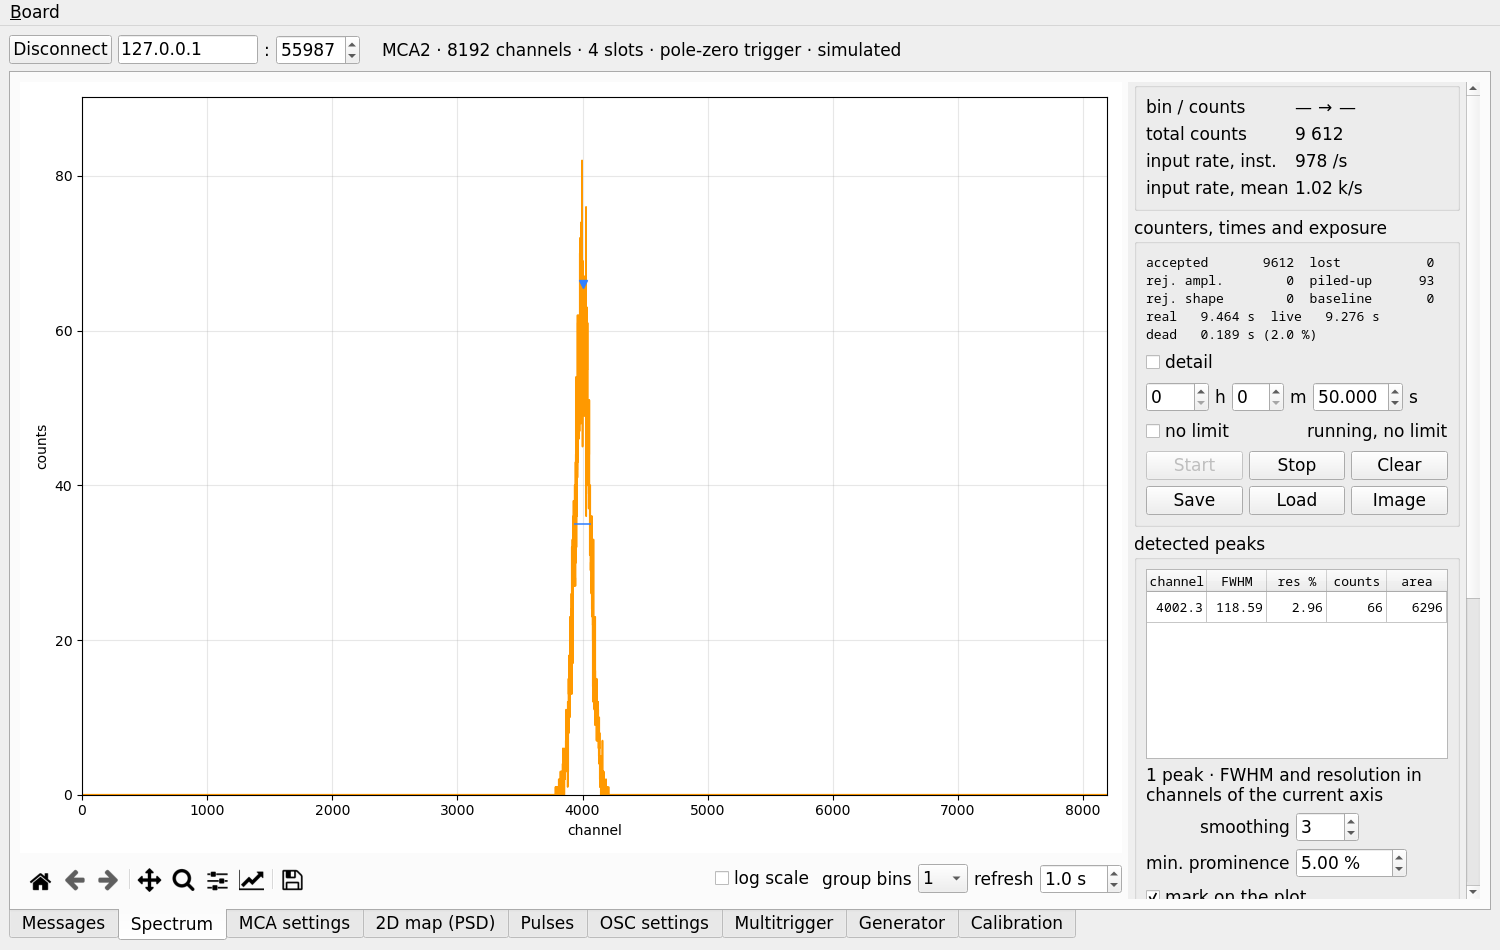
\includegraphics{apD_mcamon_spectrum}
\caption[Pestaña \emph{Spectrum}]{%
Pestaña \emph{Spectrum}: el histograma 1D con los contadores, los tiempos, los
controles de la adquisición y la lista de picos
detectados.\label{f:ap-app-spectrum}}
\end{figure}

En la Fig.~\ref{f:ap-app-2d-map} se presenta la pestaña 2D \emph{map} (PSD): el mapa de
amplitud $\times$ factor de forma ($Q_\text{tail}/Q_\text{total}$), con las
cuentas en escala logarítmica. En la captura, el MCA simulado genera dos
poblaciones de pulsos con la misma amplitud y distinta forma, que en el mapa
aparecen como dos manchas separadas a lo largo del eje del factor de forma. A la
derecha se calcula la figura de mérito (FOM) de esa separación, sobre la franja
de amplitudes que se elija.

\begin{figure}[H]
\centering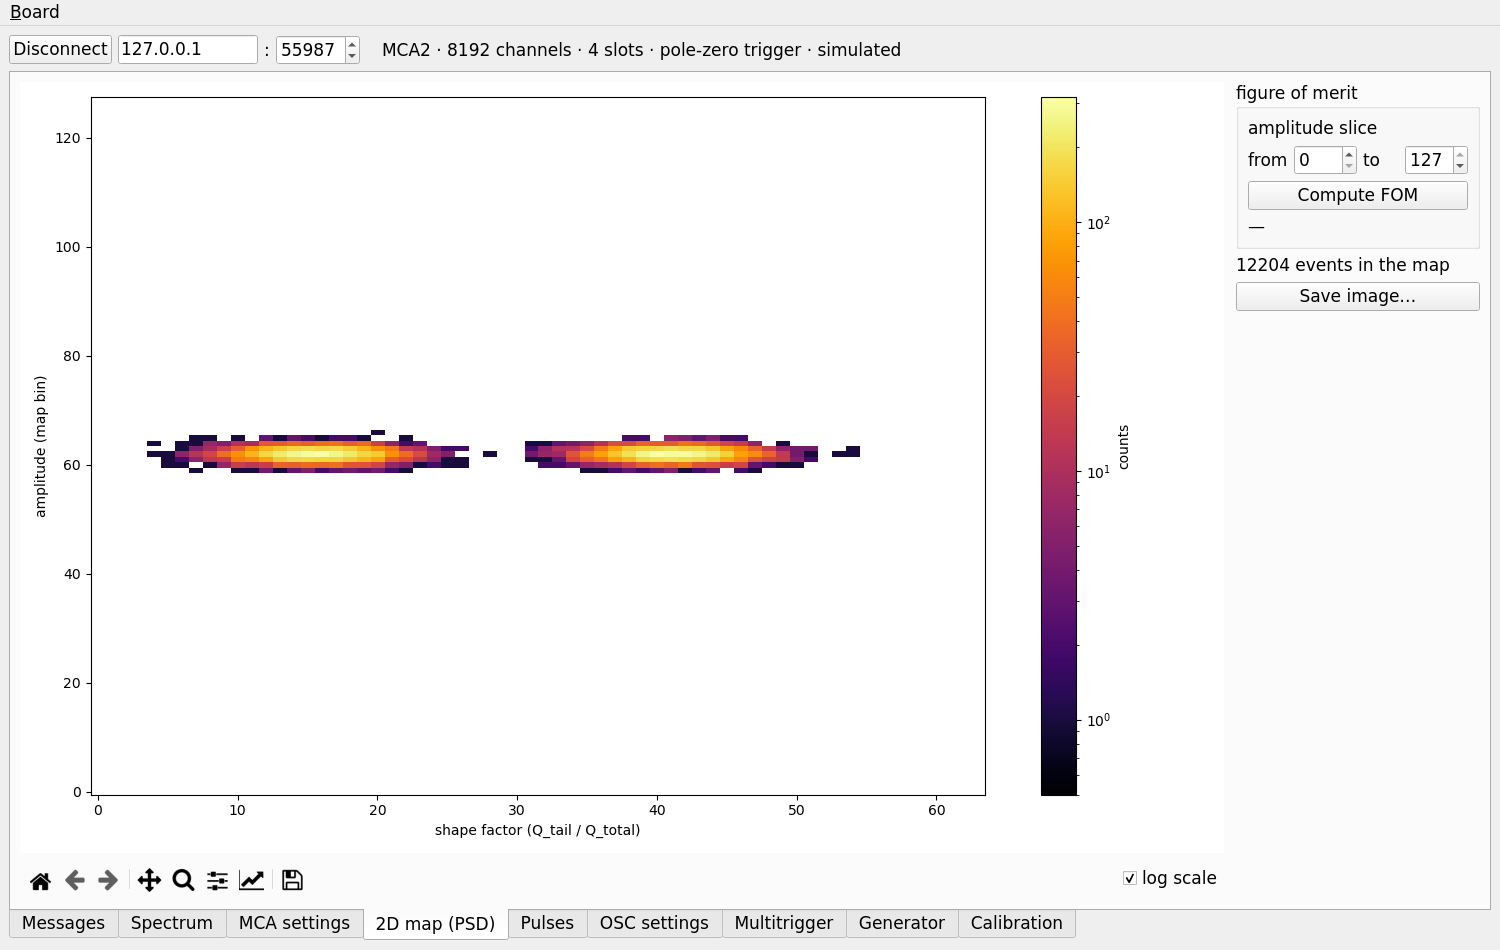
\includegraphics{apD_mcamon_2d_map_psd}
\caption[Pestaña 2D \emph{map} (PSD)]{%
Pestaña 2D \emph{map} (PSD): el mapa de amplitud $\times$ factor de forma con dos
poblaciones de pulsos simuladas, y el cálculo de la figura de mérito sobre una
franja de amplitudes.\label{f:ap-app-2d-map}}
\end{figure}

En la Fig.~\ref{f:ap-app-pulses} se presenta la pestaña \emph{Pulses}. Arriba está la
última captura del osciloscopio en IN1 e IN2, en volts contra el tiempo desde el
disparo, con la persistencia de las capturas anteriores; a la derecha se eligen
las muestras antes y después del disparo, la captura continua y la vista (pulso
o mapa de calor). Abajo está la tasa en el tiempo: los eventos aceptados por el
MCA, su media y los disparos del OSC. La línea vertical punteada marca en qué
momento de esa curva se tomó la captura de arriba.

\begin{figure}[H]
\centering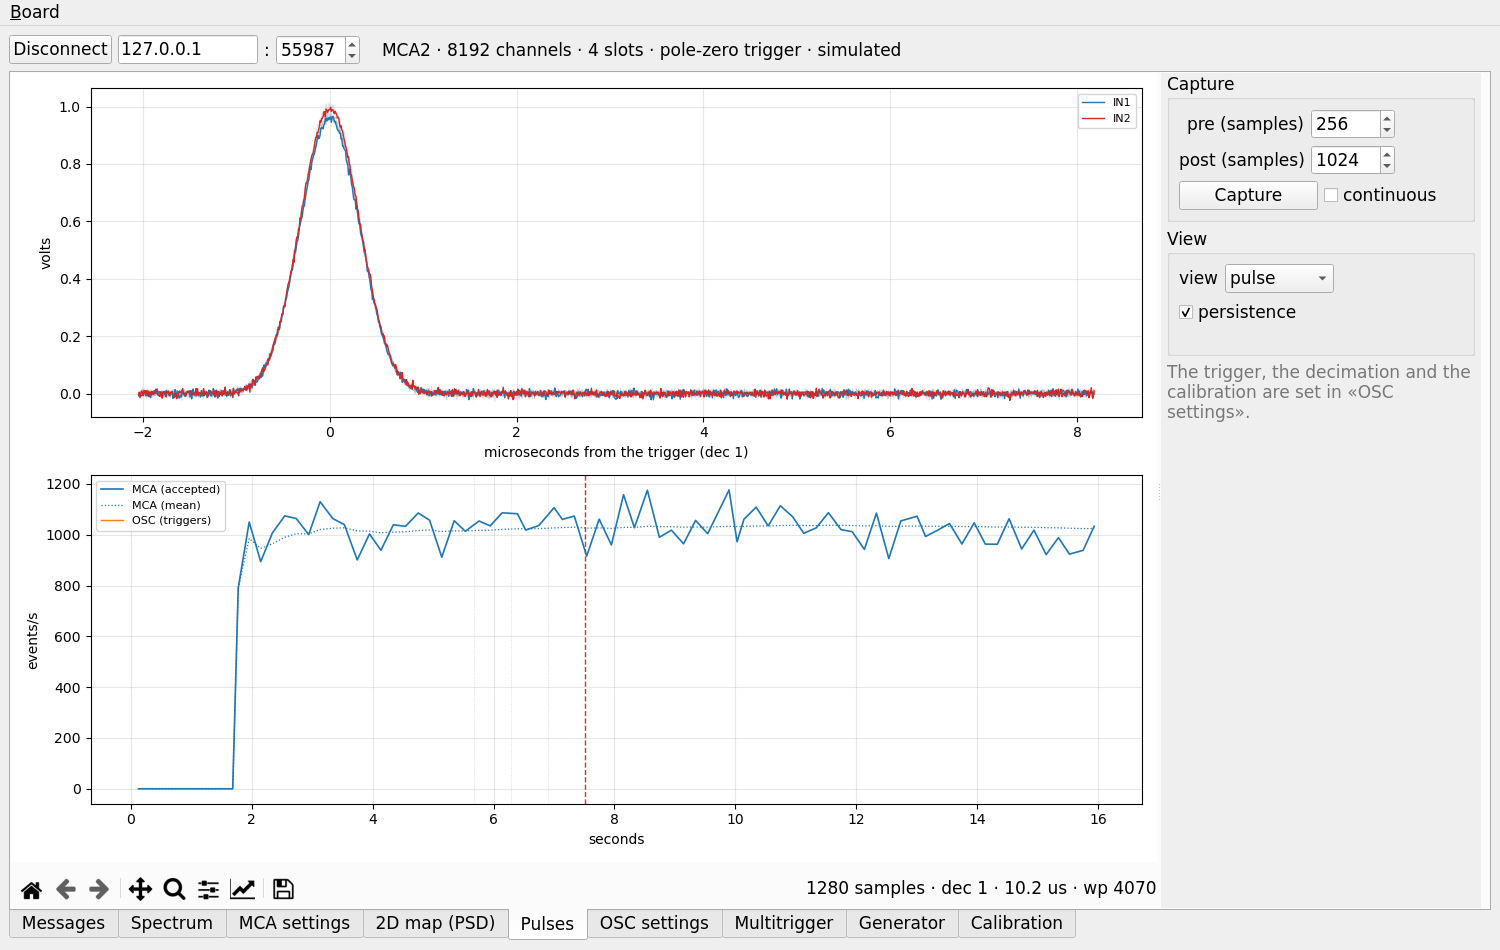
\includegraphics{apD_mcamon_pulses}
\caption[Pestaña \emph{Pulses}]{%
Pestaña \emph{Pulses}: arriba, la última captura del osciloscopio en IN1 e IN2; abajo,
la tasa de eventos en el tiempo, con el momento de la captura
marcado.\label{f:ap-app-pulses}}
\end{figure}

A continuación presentamos las pestañas de configuración del MCA,
del OSC, del multitrigger, del generador de pulsos y de calibración, y la de
mensajes. Las pestañas de configuración comparten la misma organización: arriba,
una franja con el camino de los datos por etapas, con los colores del diagrama de
panorama del módulo y la tasa de cada tramo sobre su flecha; debajo de cada
etapa, en rojo, lo que se pierde o lo que deja al sistema sin eventos. Abajo, los
parámetros agrupados por etapa, cada grupo con el color de su bloque en la
franja.

En la Fig.~\ref{f:ap-app-mca-settings} se presenta la pestaña MCA \emph{settings}. La
franja recorre el MCA: la entrada (canal, decimación y retardo), la base
(seguidor automático o fija), el banco de trapezoides ---en gris, porque el
\emph{bitstream} de la captura no lo trae---, la segmentación, en la que cada disparo
del multitrigger abre una ranura, las compuertas de las ranuras y la publicación
(eje, discriminador e histograma). Bajo la segmentación se ven las pérdidas por
re-armado, por falta de ranura libre y del publicador, y bajo la publicación,
las de colisiones. Abajo, los parámetros en tres columnas: preprocesamiento
(entrada y base), segmentación y ranuras (cantidad de ranuras y compuertas \emph{short}
y \emph{long}), y publicación (eje del histograma, discriminador e histograma). La
leyenda marca qué cambios mezclan dos configuraciones en el histograma (●) y
cuáles, mal puestos, dejan el sistema sin eventos (⚠).

\begin{figure}[H]
\centering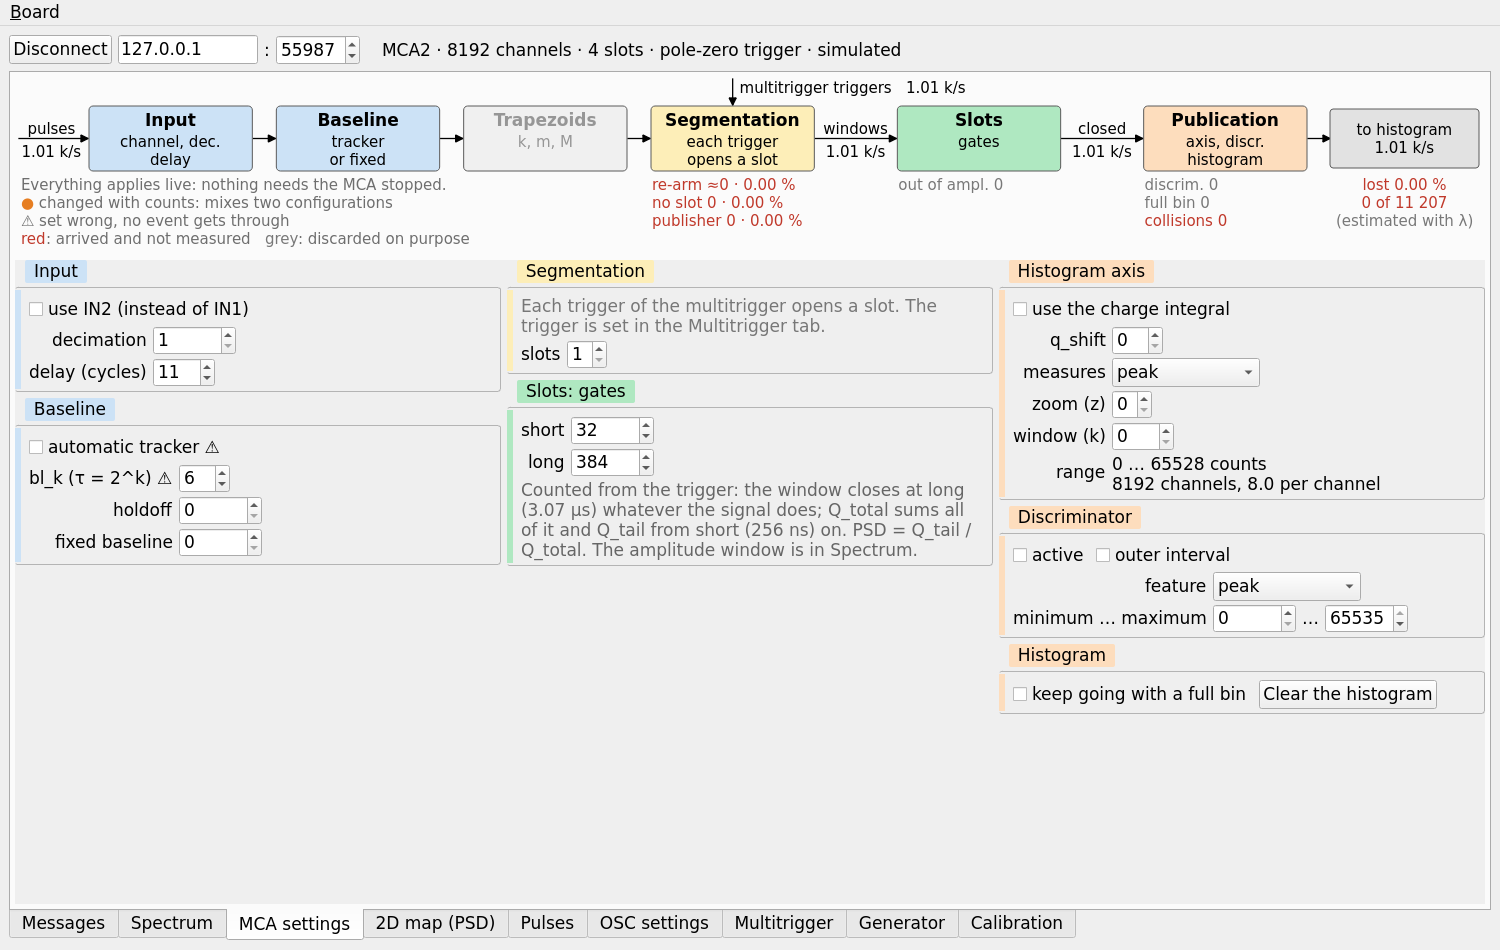
\includegraphics{apD_mcamon_mca_settings}
\caption[Pestaña MCA \emph{settings}]{%
Pestaña MCA \emph{settings}: la franja del MCA con la tasa y las pérdidas de cada
etapa, y debajo sus parámetros agrupados en preprocesamiento, segmentación y
ranuras, y publicación.\label{f:ap-app-mca-settings}}
\end{figure}

En la Fig.~\ref{f:ap-app-osc-settings} se presenta la pestaña OSC \emph{settings}. La
franja de arriba sigue al osciloscopio: la entrada (\emph{offset}, ganancia y filtro),
la decimación, el disparo que llega del multitrigger y la captura en BRAM, que
alimenta la pestaña \emph{Pulses}. La de abajo sigue al \emph{ring}, cuando el \emph{bitstream} lo
trae: el disparo o el generador de eventos abren una ventana con muestras antes y
después del disparo, que se escribe en el \emph{ring} de la DDR y se vuelca a archivos
en una carpeta de la placa. Abajo están los registros por etapa: el \emph{offset} y la
ganancia de calibración de cada canal, la decimación, el estado de la captura y
la configuración del \emph{ring} (estímulo, ventana, carpeta, formato de archivo y
memoria), con \emph{Start} y \emph{Stop} para su adquisición.

\begin{figure}[H]
\centering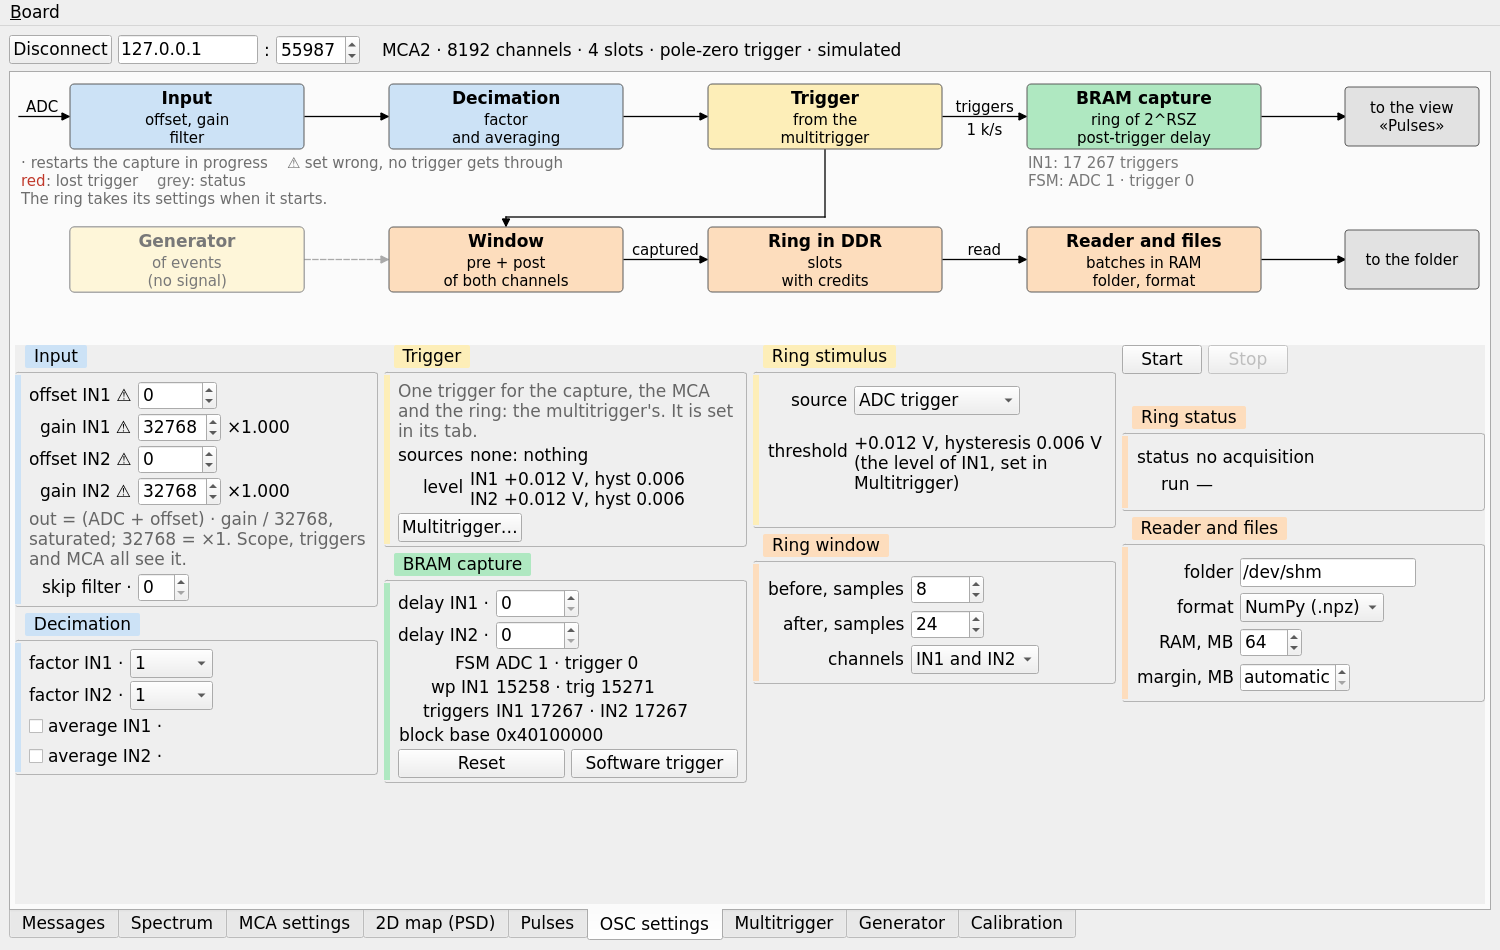
\includegraphics{apD_mcamon_osc_settings}
\caption[Pestaña OSC \emph{settings}]{%
Pestaña OSC \emph{settings}: arriba, las franjas del osciloscopio y del \emph{ring}; abajo,
los registros por etapa y la adquisición del \emph{ring} a una carpeta de la
placa.\label{f:ap-app-osc-settings}}
\end{figure}

En la Fig.~\ref{f:ap-app-multitrigger} se presenta la pestaña Multitrigger,
donde se configura el único disparo del sistema, que comparten la captura del
osciloscopio, el MCA y el \emph{ring}. La franja va desde las entradas (IN1, IN2, DIO0,
el generador y el disparo por software) a las fuentes (nivel, pendiente,
polo-cero), a la máscara OR que elige qué fuentes disparan cada canal y al
evento que llega a la captura y al MCA; debajo está el \emph{shield}, que re-arma los
canales después de un \emph{holdoff} y puede vetar al MCA. En la captura, la franja
señala en rojo que ninguna fuente está en las máscaras, así que no hay disparos.
Abajo, por etapa: los umbrales e histéresis del disparo por nivel, con su
equivalente en volts; el disparo del MCA (pendiente o polo-cero) con sus
parámetros; la grilla de la máscara, fuentes $\times$ canal y flanco; el evento;
y el \emph{shield}.

\begin{figure}[H]
\centering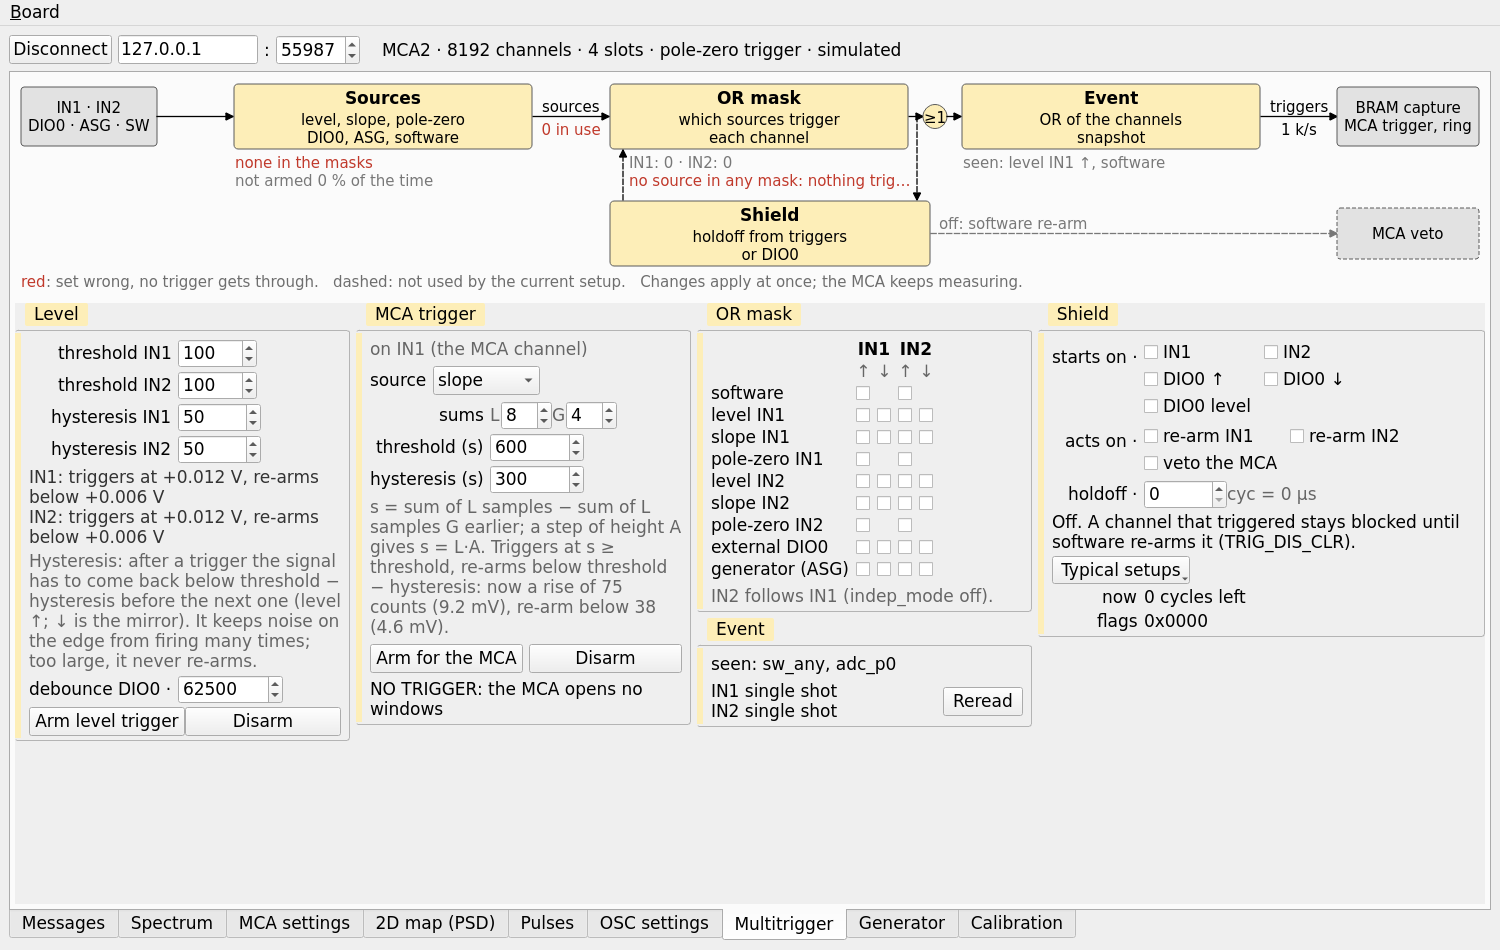
\includegraphics{apD_mcamon_multitrigger}
\caption[Pestaña Multitrigger]{%
Pestaña Multitrigger: la franja del disparo, de las entradas al evento, con el
\emph{shield}; abajo, las fuentes, la máscara OR por canal, el evento y el
\emph{shield}.\label{f:ap-app-multitrigger}}
\end{figure}

En la Fig.~\ref{f:ap-app-generator} se presenta la pestaña \emph{Generator}. La franja
sigue el orden de la ecuación del generador de pulsos,
\begin{equation}
  v(t) = B + \sum_k A_k\, h(t - t_k) + r(t),
  \label{e:ap-app-generador}
\end{equation}
con los disparos $t_k$ (periódicos o Poisson), las amplitudes $A_k$ sorteadas de
una tabla de 1024 alturas, la forma $h$ con su decaimiento $\tau_d$ y su subida
$\tau_r$, y la salida, con la base $B$, el ruido $r$ y la saturación a 14 bits,
hacia el DAC (OUT1, OUT2). Abajo están los controles de cada etapa, el lazo
digital, que lleva el generador a la entrada del MCA sin pasar por el DAC, y el
estado del generador. ``\emph{Apply}'' escribe la configuración entera y detiene el
generador.

\begin{figure}[H]
\centering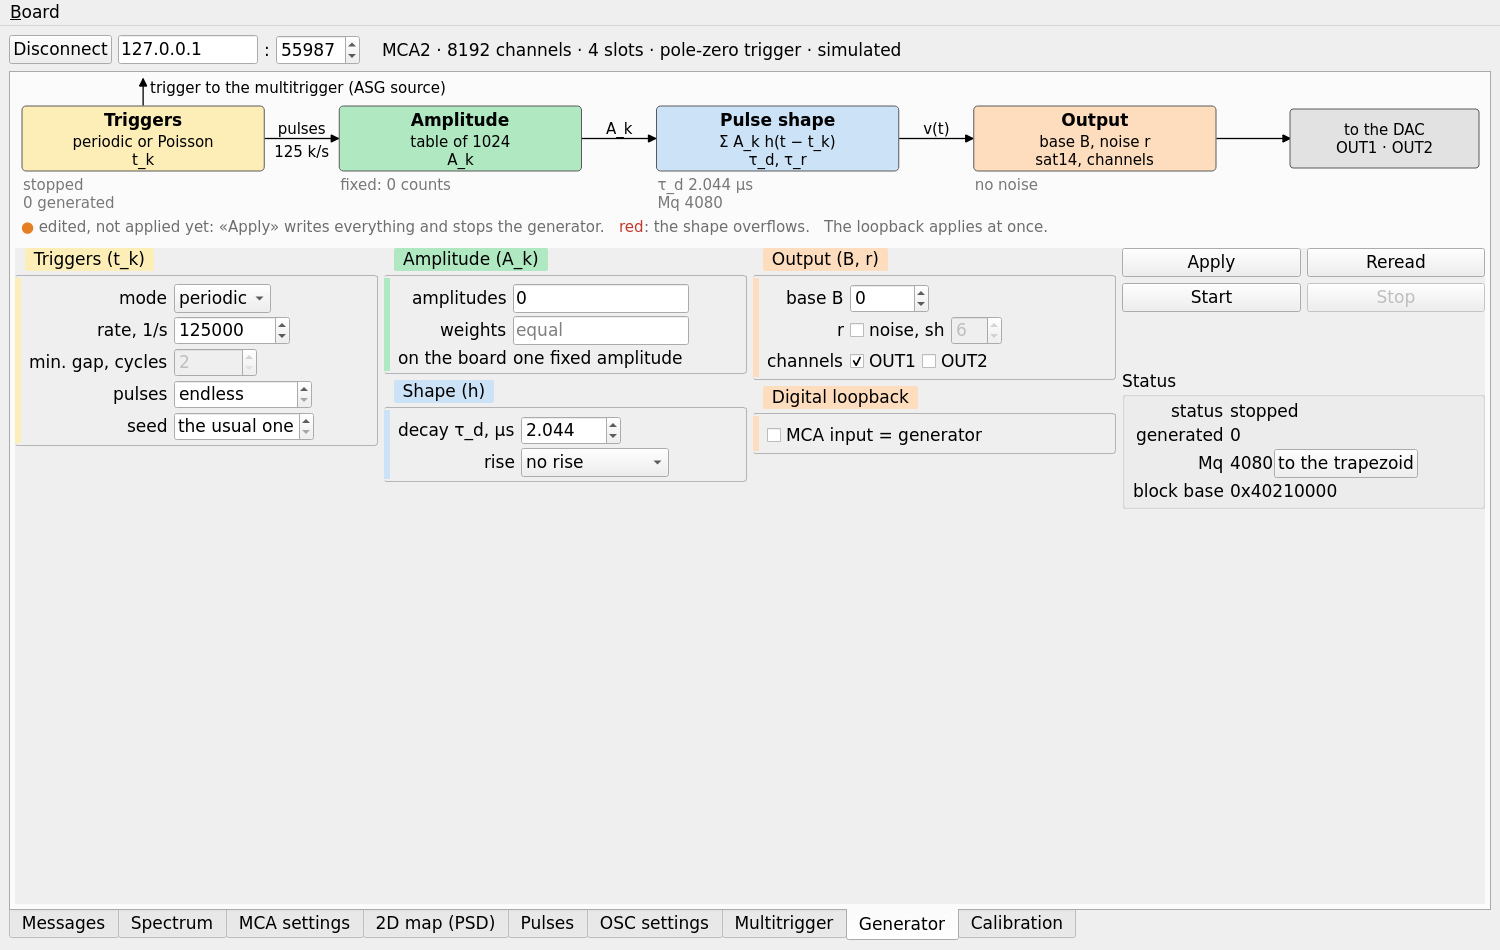
\includegraphics{apD_mcamon_generator}
\caption[Pestaña \emph{Generator}]{%
Pestaña \emph{Generator}: la franja del generador de pulsos en el orden de su
ecuación, los controles por etapa y el lazo digital hacia el
MCA.\label{f:ap-app-generator}}
\end{figure}

En la Fig.~\ref{f:ap-app-calibration} se presenta la pestaña \emph{Calibration}. La
franja va de la referencia (el generador por OUT1 o una cuadrada externa) al
canal analógico (cable, carga, \emph{front-end} y ADC), al modelo del canal (un FIR más
polos lentos, que producen una caída lenta) y a la base del MCA, fija o
dinámica. Abajo, a la izquierda, están la referencia, la conexión medida y la
tabla con el origen de la caída lenta, una fila por conexión; al centro, los
resultados (\emph{offset} y ruido, ganancia, caída lenta y por polo, latencia, subida,
ancho de banda, residuo y diafonía) y la configuración de la base del MCA; a la
derecha, la respuesta al escalón rápida y lenta, la respuesta en frecuencia del
FIR, el piso de ruido de IN1 y la variación de la base dinámica en el último
minuto. Los valores de la captura salen del canal simulado.

\begin{figure}[H]
\centering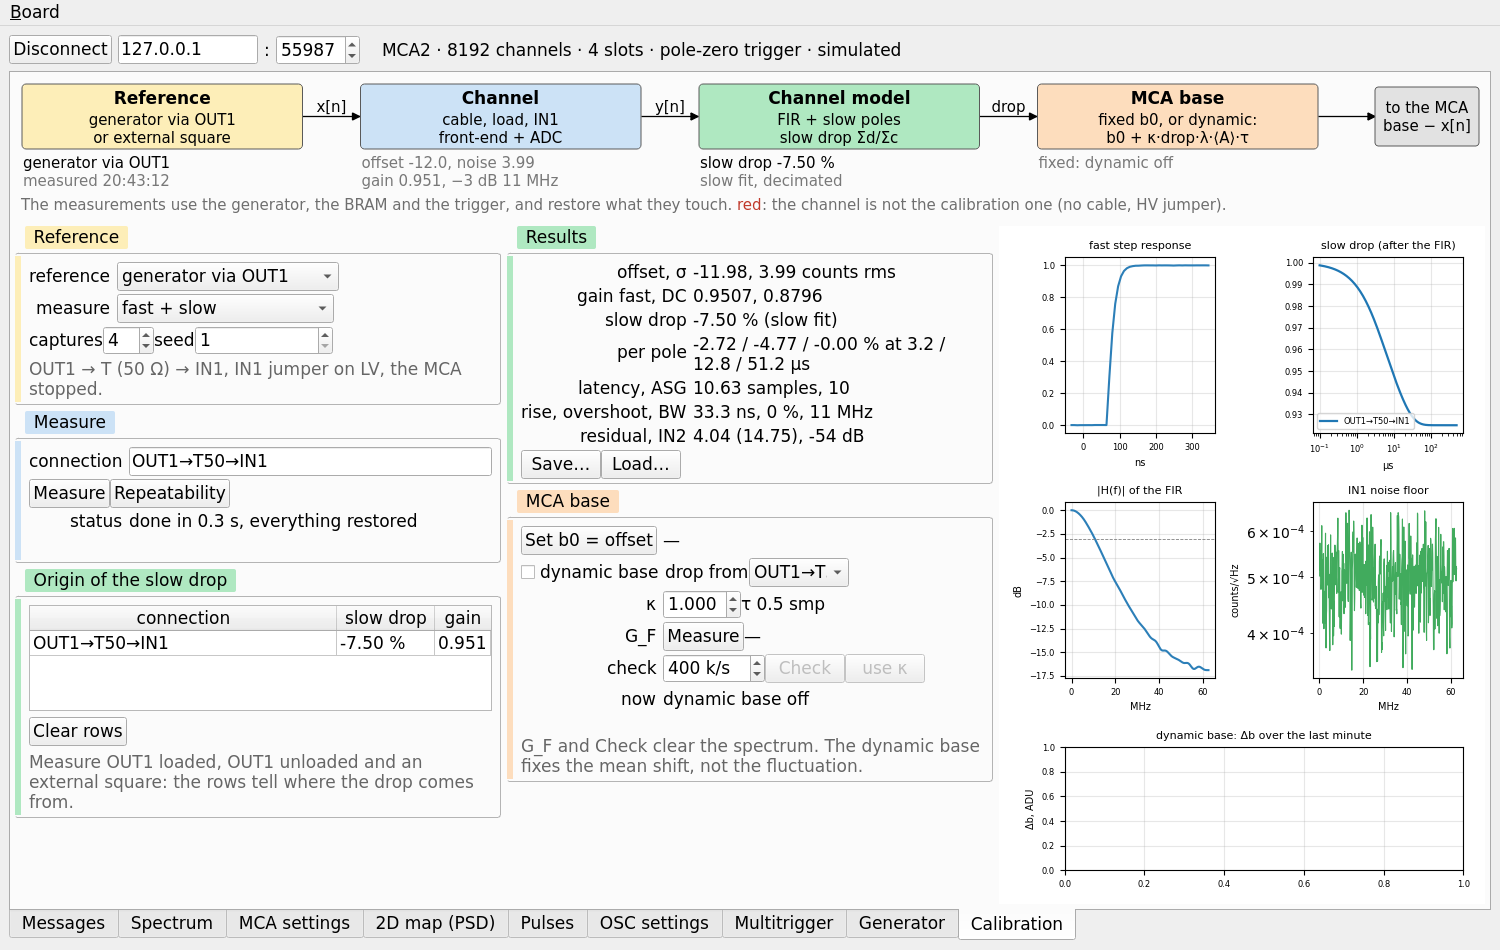
\includegraphics{apD_mcamon_calibration}
\caption[Pestaña \emph{Calibration}]{%
Pestaña \emph{Calibration}: la medición del canal analógico con una referencia
conocida, sus resultados, el origen de la caída lenta y la base del
MCA.\label{f:ap-app-calibration}}
\end{figure}

En la Fig.~\ref{f:ap-app-messages} se presenta la pestaña \emph{Messages}, que
registra cada operación y cada error con su hora. En la captura se ven la
conexión al MCA simulado, con la cantidad de canales y si el \emph{bitstream} trae el
mapa 2D, y el arranque de la adquisición. El registro se puede guardar en un
archivo con ``\emph{Save log}…''.

\begin{figure}[H]
\centering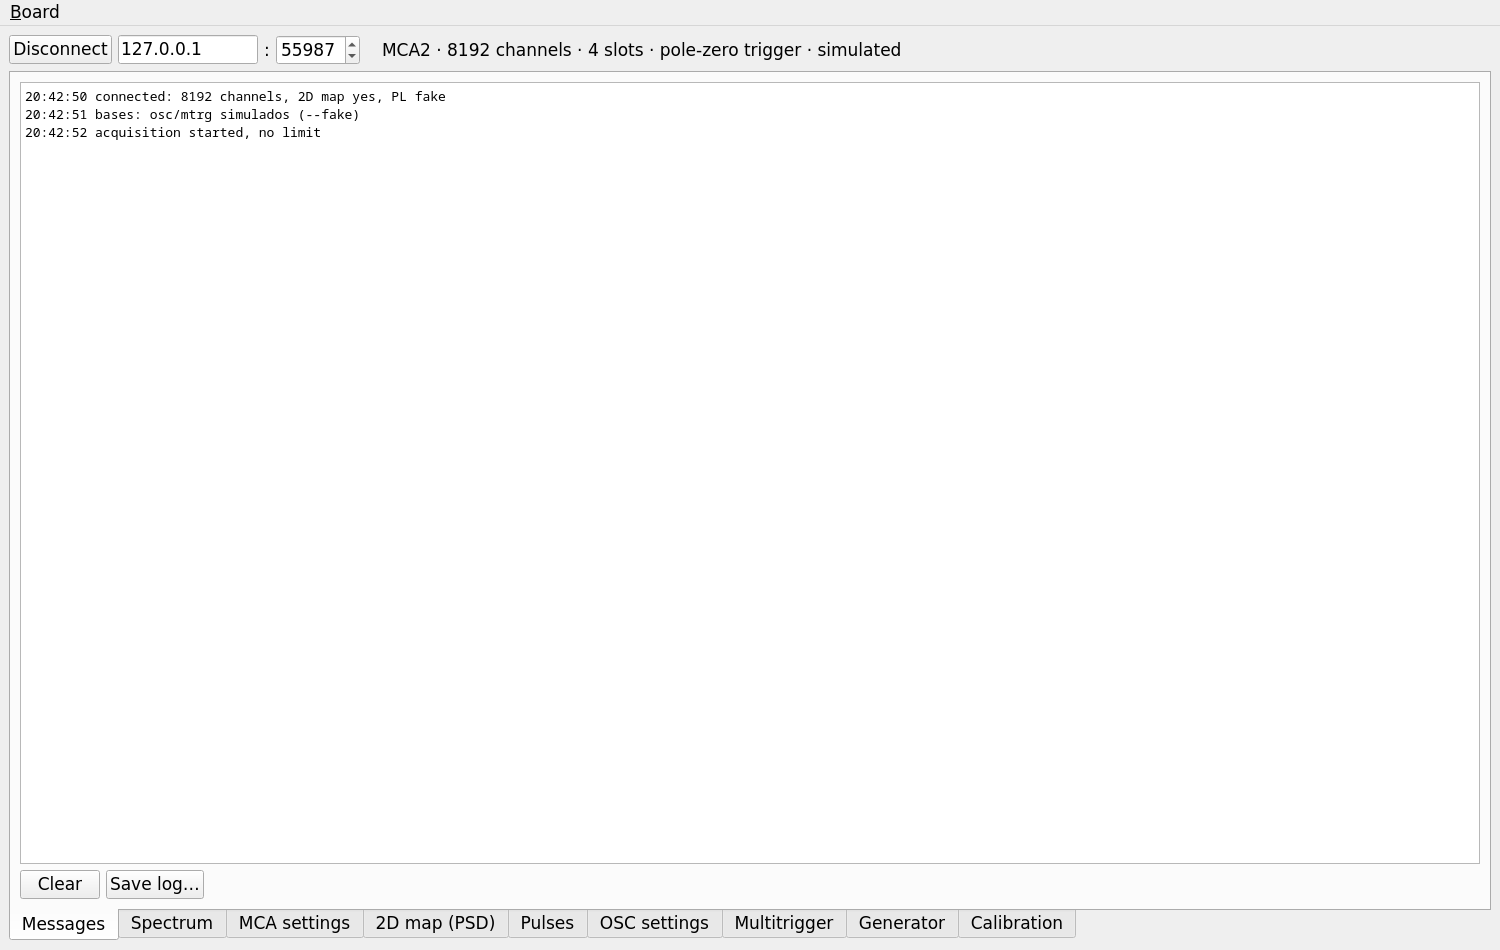
\includegraphics{apD_mcamon_messages}
\caption[Pestaña \emph{Messages}]{%
Pestaña \emph{Messages}: el registro de operaciones y errores, con su
hora.\label{f:ap-app-messages}}
\end{figure}

%%% Local Variables:
%%% mode: latex
%%% TeX-master: "template"
%%% End:
